\subsection{Total dephasing in the selective regime}
\label{subsec:total_dephasing_selective}

Operating at the selective-regime sweet spot protects the cavity states
$\lvert g,m^\star\rangle$--$\lvert g,m^\star\!+\!1\rangle$ from flux-noise dephasing.
Under drive, however, the residual dephasing budget in the selective regime is set by two
contributions: (i) cavity pure dephasing at a rate
$\gamma_{c\phi}^{\mathrm{sel}}=\bigl(g^2/\Delta_{bc}^2\bigr)\gamma_{b\downarrow}$,
arising from the Purcell-like mixing of cavity and FTT decay channels, and
(ii) FTT heating at a rate $\gamma_{b\uparrow}^{\mathrm{sel}}\propto 1/\lvert\Delta_{bd}\rvert$
induced by photon shot noise (see App.~\ref{Linbladian regime} for derivations). Because the shot-noise contribution scales unfavorably as $1/\lvert\Delta_{bd}\rvert$, operating at larger detuning—i.e., in the unselective regime—yields a lower total dephasing rate.

\subsection{Numerical evaluation of the total dephasing rate}
\label{subsec:numerical_total_dephasing_rate}

Full-system simulations are used to extract the cavity dephasing rate under drive; the
numerical procedure and fitting protocol are summarized in App.~\ref{app:dephasing_numerics}.
The noise amplitude $S_0$ and the detuning $\Delta_{bd}$ are sampled over the parameter
range of interest. For each $\Delta_{bd}$, the drive amplitude is chosen to satisfy the
sweet-spot condition, and the corresponding total dephasing rate
$\Gamma_{\phi,\mathrm{total}}$ is extracted.

Fig.~\ref{fig:total_rate}(a) summarizes the results. For $S_0=10^{-5}/\Phi_0$, the
drive-induced contribution $\gamma_{b\uparrow}^{1/f,\mathrm{un}}$ dominates
$\Gamma_{\phi,\mathrm{total}}$ over the scanned detuning range. At large detuning,
$\lvert\Delta_{bd}\rvert> \lvert\chi\rvert\simeq 2~\mathrm{MHz}$, the total rate is well described by $\gamma_{b\uparrow}^{1/f,\mathrm{un}}$, which is independent of the detuning. At smaller detuning, i.e.\
$-\Delta_{bd}/2\pi=1~\mathrm{MHz}<\lvert\chi/2\pi\rvert$, the rate
increases as the dynamics enters the selective regime, consistent with the
$1/\lvert\Delta_{bd}\rvert$ scaling.

For smaller noise amplitude, e.g.\ $S_0=10^{-6}/\Phi_0$, the $S_0$-independent drive-induced contributions
$\gamma_{b\uparrow}^{\mathrm{un}}$ and $\gamma_{c\phi}^{\mathrm{un}}$ dominate
$\Gamma_{\phi,\mathrm{total}}$. At large detuning ($-\Delta_{bd}/2\pi=19~\mathrm{MHz}$),
$\gamma_{b\uparrow}^{\mathrm{un}}\propto(\Delta_{bd}/K)^2$ dominates while
$\gamma_{c\phi}^{\mathrm{un}}\sim K/\Delta_{bd}$ is suppressed; the opposite hierarchy
holds at small detuning ($-\Delta_{bd}/2\pi=1~\mathrm{MHz}$). Consequently,
$-\Delta_{bd}/2\pi=6~\mathrm{MHz}$ yields the minimal $\Gamma_{\phi,\mathrm{total}}$
within the scanned range. In the undriven case, the dephasing time is
$\sim 0.1$--$1~\mathrm{ms}$ as $S_0$ varies from $10^{-5}/\Phi_0$ to $10^{-6}/\Phi_0$. With $\Delta_{bd}/2\pi\simeq -6~\mathrm{MHz}$ and
sweet-spot driving, the dephasing time improves by up to $\sim 20\times$ across the
considered $S_0$ range, confirming the overall dephasing enhancement.

\begin{figure}[t]
    \centering
    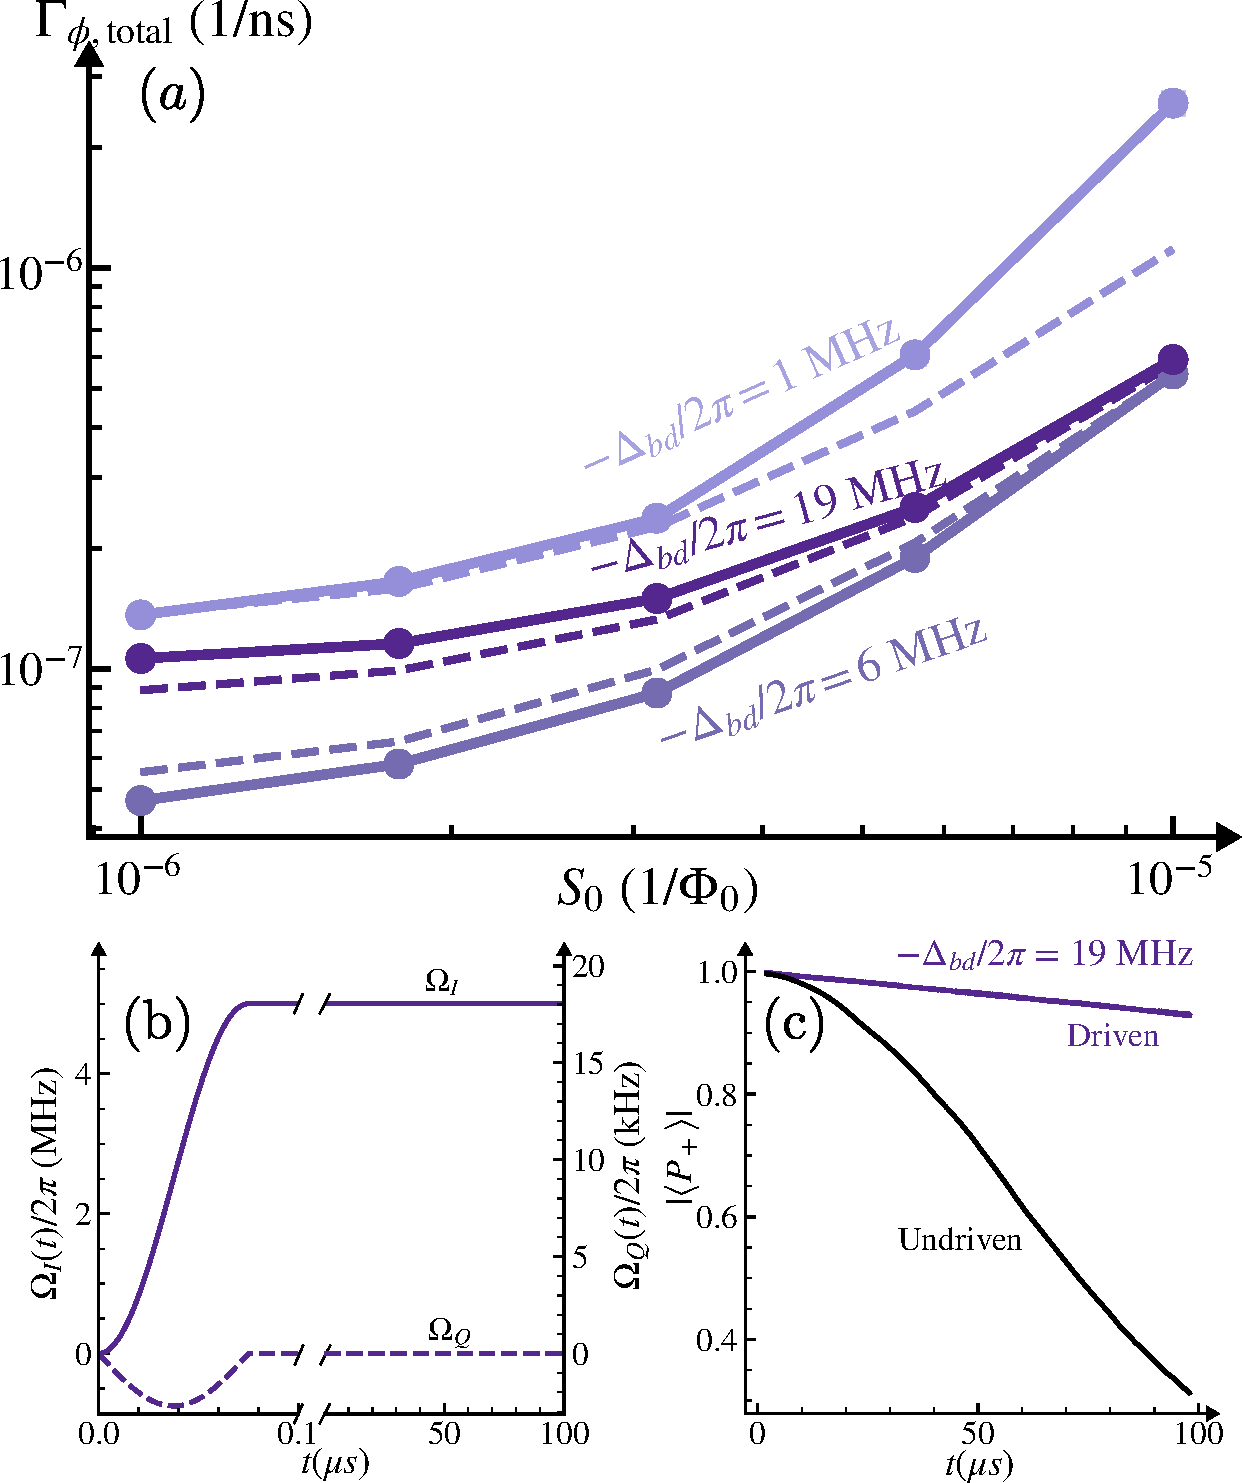
\includegraphics[width=\linewidth]{Sec 3/total_rate.pdf}
    \caption{Numerical evaluation and time-domain validation of the total cavity dephasing
    rate under sweet-spot driving. (a) Total dephasing rate $\Gamma_{\phi,\mathrm{total}}$
    extracted from full-system simulations as a function of detuning $\Delta_{bd}$, with
    the drive amplitude chosen at each detuning to satisfy the sweet-spot condition.
    $S_0$ denotes the amplitude of $1/f$ flux noise. (b) DRAG-style adiabatic ramp pulse.
    (c) Time-domain decay of
$P_X(t)=\mathrm{Tr}\!\left[\rho(t)\,X(t)\right]$, with
$X(t)=\ket{\phi_{g,1}(t)}\!\bra{\phi_{g,0}(t)}+\mathrm{H.c.}$.
The time-dependent Floquet states are labeled by their bare-state correspondence.
The driven system exhibits a cavity dephasing time of $\sim 2~\mathrm{ms}$,
compared to $\sim 100~\mu\mathrm{s}$ in the undriven case.}
    \label{fig:total_rate}
\end{figure}

To visualize the dephasing enhancement directly, we perform time-domain simulations that
include relaxation and stochastic flux noise with $S_0=10^{-5}/\Phi_0$. The initial state is
$\ket{\psi_0}=\tfrac{1}{\sqrt{2}}\big(\ket{g,0}+\ket{g,1}\big)$. With drive, the state is
adiabatically mapped onto the target Floquet states using a shaped pulse
$2\Omega_0(t)\cos\!\big(\omega t+\phi(t)\big)$. In the rotating frame this yields the
$I$ and $Q$ quadratures
\begin{align}
\Omega_I(t) = \Omega(t)\cos\phi(t), \qquad
\Omega_Q(t) = \Omega(t)\sin\phi(t).
\end{align}
We implement a DRAG correction,
$\Omega_Q(t) = -\dot{\Omega}_I(t)/\Delta_{bd}$, which accelerates the adiabatic transfer
relative to $\Omega_I(t)$-only ramps (see App.~\ref{Adiabatic transition}). A pulse ramp
with $\tau=75~\mathrm{ns}$ is shown in Fig.~\ref{fig:total_rate}(b).

The dephasing is quantified by the coherence operator
\begin{align}
X(t) &= \ket{\phi_{g,1}(t)}\!\bra{\phi_{g,0}(t)} + \mathrm{H.c.}, \\
P_X(t) &= \mathrm{Tr}\!\left[\rho(t)\,X(t)\right],
\end{align}
where $\ket{\phi_{g,1}(t)}$ and $\ket{\phi_{g,0}(t)}$ are adiabatically mapped from the bare states.
Without drive, \(1/f\) noise produces sub-Gaussian free-induction decay. At the driven sweet spot, the dominant residual channel is Markovian, arising from FTT depolarization, and yields the exponential decay observed in Fig.~\ref{fig:total_rate}(c). The dephasing time \(T_2\) is extracted from an exponential fit to \(P_X(t)\) (see Appendix I). Under sweet-spot driving, the dephasing time reaches \(\sim 2~\mathrm{ms}\), compared with \(\sim 100~\mu\mathrm{s}\) in the undriven case.